% arara: lualatex
% !TEX TS-program = LuaLaTeX

\documentclass{coderdojo}


\worksheet{3}{Graphical Take Away}

\begin{document}
\maketitle

\section*{Introduction}

In the previous worksheet, we created a text based version of the Take Away game:

\begin{exercise}[title=Take Away Game]
Game consists of a pile of coins with two players taking turns to play. At each turn the player decides to take 1, 2 or 3 coins.  The player who take the last coin wins.

\centerline {\includegraphics[page=12]{take_away_game}}
\end{exercise}

We would like to now create a graphical version of this game but there are a few concpets we need to cover first. In particular:

The competed text-based version of the game is included in the next page. In order to create a graphical version we will need to cover some additional concepts.

\begin{dingautolist}{192}
\item \hyperref[sec:turtle]{\color{section}\bfseries Turtle graphics}

Turtle graphics is a python module that allow us to create drawings   It was designed to help teach 
programming concepts so is similar to Scratch programming. 

\item \hyperref[sec:event]{\color{section}\bfseries Event programming}

We will cover a programming style that is more suited to graphical programs.

\item \hyperref[sec:game]{\color{section}\bfseries  Designing our Game}

OK, now we return to our game and design our graphic version.

%\item \hyperref[sec:event]{\color{section}\bfseries  }

\end{dingautolist}

\codeonly{title={Completed \code{TakeAway.py} from Chapter 2}}{1}{200}{code}{TakeAway.py}

\section{Turtle graphics}

Turtle graphics is centred around the idea of little turtles that we can control and as they move they trace out a path. The idea is simple, but it is surprising simple to create complex pictures. It was used to develop programming languages such as LOGO which ultimately led to Scratch.

To get us started let's write a few small programs demonstrating its capabilities \ldots

\begin{itemize}
\item[\todoSymbol] \color{todo}
Create a new file with the following code and save as \code{first.py}.
\end{itemize}

\codeandoutput{title={\code{first.py}}}{1}{6}{code}{first.py}{%
	\centering	
	\tikz\node[fill=white]{
	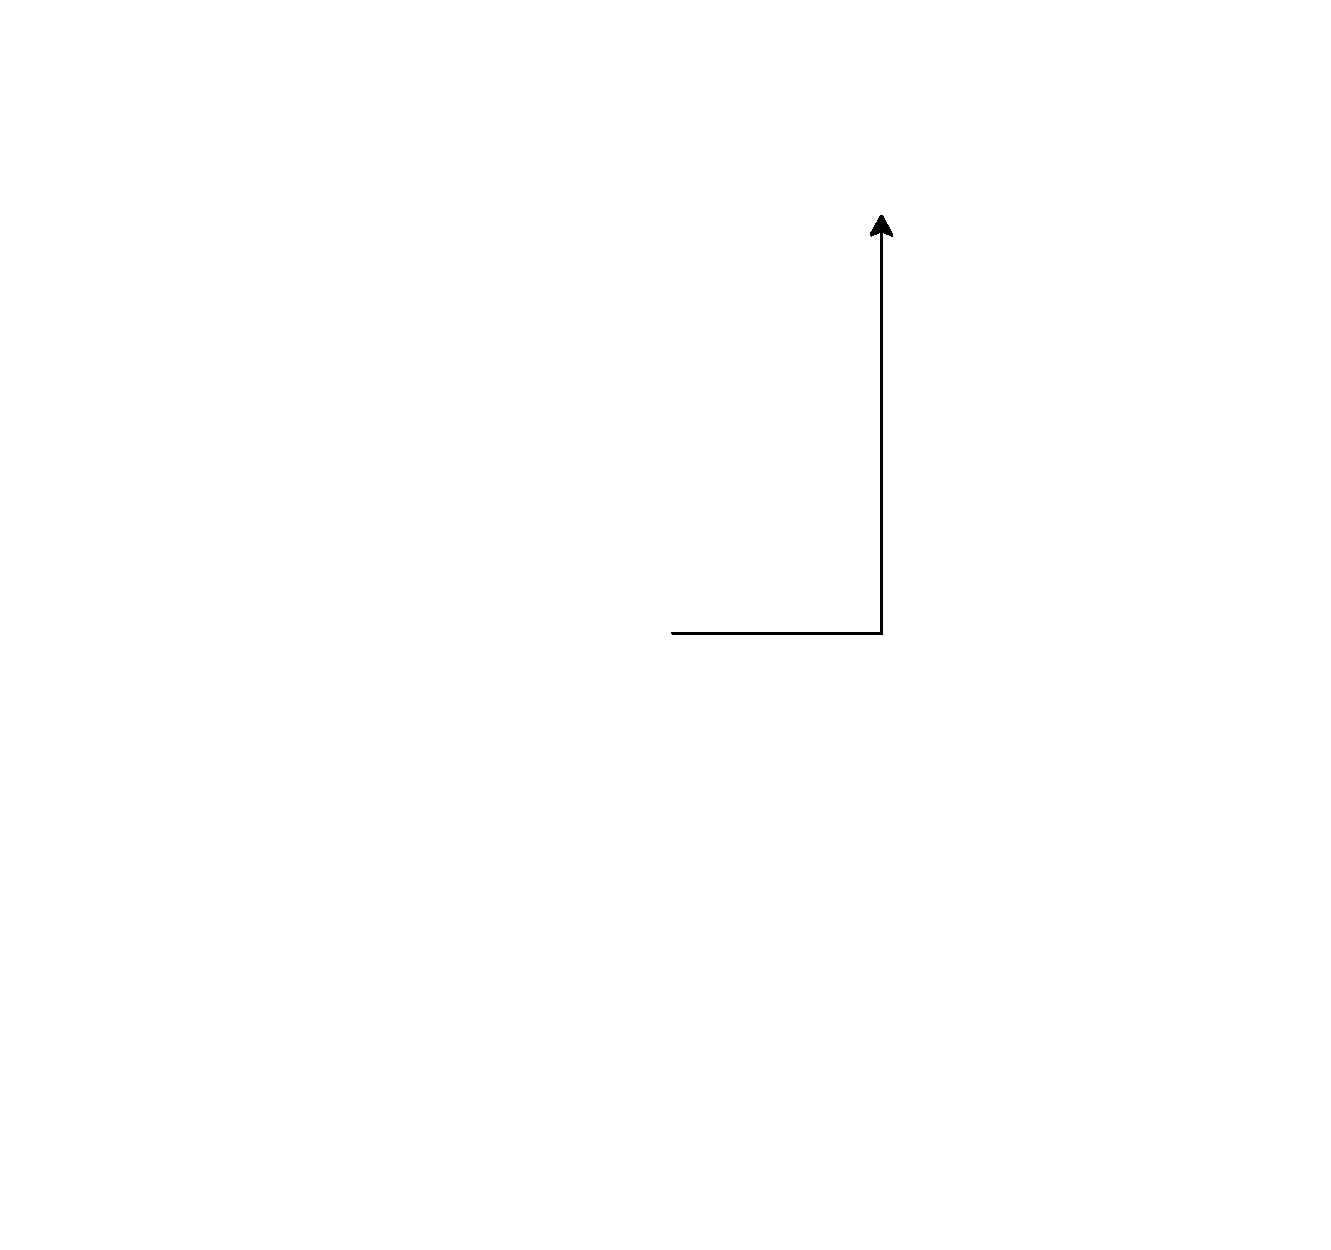
\includegraphics[clip,trim=0 200 0 100, width=\textwidth]{code/first.pdf}};
}

\begin{itemize}
\item[\pointSymbol]
 In line 1, we import the turtle module. This gives us access to all of the commands defined in this module. Remember we also used this command to import the \code{random} module previously.
\item[\pointSymbol]
Next we create a new turtle (pen) and we call it \code{bob}. We could use any name here. I like bob because it is nice and short, so saves on the typing.
 
\item[\pointSymbol]
In the remaining lines we tell \code{bob} what to do and \code{Bob} happily (i hope) does it.
\code{bob} understands a large number of commands, including\\

{\bfseries\color{section} Movement commands}
\begin{itemize}
\item \code{forward} --- move forward a given distance.
\item \code{backward} --- move backward a given distance.
\item \code{left} --- turn left a given angle (measured in degrees)
\item \code{right} --- turn right a given angle (measured in degrees)
\item \code{setheading} --- turn to face in a given direction.
\item \code{setposition} --- move to a given position (horizontal and vertical.
\begin{itemize}
\item \code{setx} --- move to a given horizontal position.
\item \code{sety} --- move to a given vertical position.
\end{itemize}
\item \code{home} --- move back to starting position and direction
\end{itemize}

{\bfseries\color{section} Drawing commands}
\begin{itemize}
\item \code{dot} --- draw a dot of given radius in current position
\item \code{circle} --- draw a circle of given radius in current position
\item \code{penup} --- "lifts pen" so subsequent movement will not be drawn.
\item \code{pendown} --- "lowers pen" so subsequent movement will be drawn.
\item \code{color} --- set the drawing colour. Use a known colour such as \code{"red"} or by building your own by mixing the primary colours (red, green and blue).
\item \code{stamp} --- stamp a copy of the turtle shape at the current turtle position.
\item \code{write} --- write a message to the screen.
\end{itemize}
{\bfseries\color{section} Control commands}
\begin{itemize}
\item \code{speed} --- set how fast the turtle moves:  \code{"slowest"}, \code{"slow"}, \code{"normal"}, \code{"fast"}, and  \code{"fastest"}.
\item \code{undo} ---undo (repeatedly) the last turtle action(s).
\item \code{clearstamp} --- delete a perviously placed stamp.
\end{itemize}
\end{itemize}

\subsection{Drawing Shapes}

Just listing commands for the turtle to do is great and all that but the magic really happens when we use repetition  (\code{for} and \code{while} loops) and decisions (\code{if}--\code{elif}--\code{else} statement) to build more complicated diagrams with only little effort from us, the programmer.


\begin{itemize}
\item[\todoSymbol] \color{todo}
Create a new file with the following code and save as \code{Square_Basic.py}.
\end{itemize}

\codeandoutput{title={\code{Square_Basic.py}}}{1}{10}{code}{Square_Basic.py}{%
	\centering	
	\tikz\node[fill=white]{
	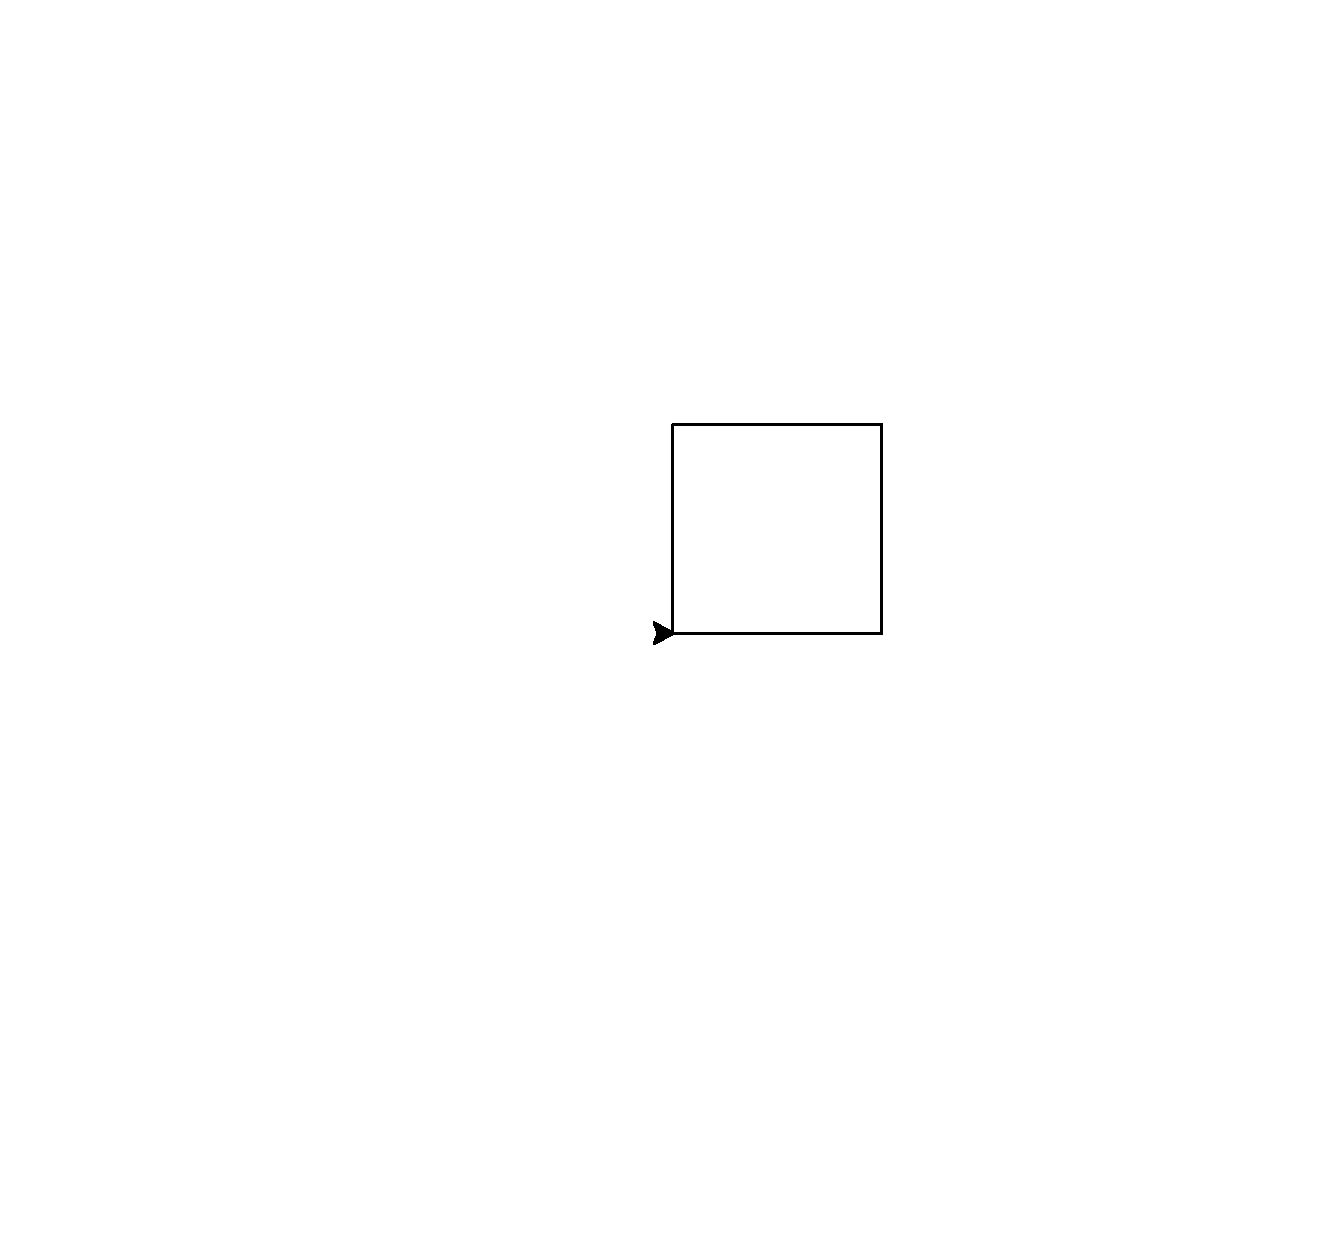
\includegraphics[clip,trim=100 150 100 150, width=\textwidth]{code/Square_Basic.pdf}};
}

OK, the generated diagram was (hopefully) not a surprise --- a square is just four lines of equal length joined by 90$^\circ$ angles. But our code is getting long and, worse, it is getting repetitive. Let's fix that with a \code{for} loop.

\begin{itemize}
\item[\todoSymbol] \color{todo}
Create a new file with the following code and save as \code{Square_Loop.py}.
\end{itemize}

\codeandoutput{title={\code{Square_Loop.py}}}{1}{10}{code}{Square_Loop.py}{%
	\centering	
	\tikz\node[fill=white]{
	\includegraphics[clip,trim=100 150 100 150, width=\textwidth]{code/Square_Loop.pdf}};
}

OK, the code is not that much shorter. But it no longer repetitive! it is a big deal when we want to write good code.


\begin{itemize}
\item[\todoSymbol] \color{todo}
Create a new file, save it as \code{Triangle.py} which draws a triangle.
\item[\todoSymbol] \color{todo}
Create a new file, save it as \code{Pentagon.py} which draws a pentagon.
\end{itemize}

\clearpage

The steps for drawing the triangle, square and pentagon are similar --- so again to avoid repetitive code --- we could identify the pattern and write a function for this \ldots 
\begin{itemize}
\item[\todoSymbol] \color{todo}
Create a new file with the following code and save as \code{Polygon.py}.
\end{itemize}

\codeandoutput{breakable,title={\code{polygon.py}}}{1}{100}{code}{polygon.py}{%
	\centering	
	\tikz\node[fill=white]{
	\includegraphics[clip,trim=150 200 50 0, width=\textwidth]{code/polygon.pdf}};
}


We will talk in class and if you like we play with turtle graphics a while to see what we can generate. for example, I really like the following 
 
\codeandoutput{breakable,title={\code{spiral.py}}}{1}{100}{code}{spiral.py}{%
	\centering	
	\tikz\node[fill=white]{
	\includegraphics[clip,trim=0 0 0 0, width=\textwidth]{code/spiral.pdf}};
}

\clearpage
\section{Event programming}

Today we are going to write our programmes using a different style or {\bfseries programming paradigm} called {\bfseries event programming}

\begin{asideBox}[colbacktitle=section!50,drop shadow, watermark tikz={\draw[line width=2mm] circle (1cm)
            node{\fontfamily{ptm}\fontseries{b}\fontsize{20mm}{20mm}\selectfont i};}]{Programming Paradigms}

{\bfseries Programming paradigms} is not about using different programming languages but about different ways of structuring our code.  Picking the right programming paradigms can have a huge impact on the effort needed to implement a task.  So far we have used {\bfseries imperative programming} but there are many others \ldots

\begin{itemize}
\item[\color{section}\larger\ding{237}]
{\bfseries Imperative programming} is a programming style where we write a sequence of commands in a particular order that the computer must execute in that order.  Essentially, we are telling the computer ``do this \ldots\ do this \ldots\ do this \ldots\ do this \ldots\ do this \ldots''

	{\smaller\it  Imperative programming is a very common style and because we decide on the order commands are executed it can be easier to debug.}
	
\item[\color{section}\larger\ding{237}] 
{\bfseries Event programming} is a programming style where we write separate blocks of code, usually functions, and we tell the computer to listen/watch for events to happen. An event could be a key pressed, or a message received across the internet, etc.  With each event we link it to one of our blocks of code. 

 Whenever a listed event occurs the computer tries to interrupt what it is doing and run the linked code immediately, and then resume its previous task. 

	{\smaller\it  Because the programmer does not control what event occur, the programmer does not know the order their commands will be executed.  This can make writing/debugging event programming code more difficult. However, event  programming is ideal for programs that have a graphical interface with the user..}
	
\item[\color{section}\larger\ding{237}]  
{\bfseries Object oriented programming} is a programming style where we group data and code into an {\bfseries object}. This is useful because often only certain tasks make sense to be applied to certain data. 

	{\smaller\it  This paradigm is popular for developing large programs or for programs that will be used a part of developing other programs.}
	
\item[\color{section}\larger\ding{237}]  and many, many more \ldots

Some programming languages are designed around one programming paradigm, but python support many. You, the programmer, can decide which paradigm to use, and often mix style to suit the task at hand.
\end{itemize}

\end{asideBox}

\clearpage
\begin{itemize}
\item[\todoSymbol] \color{todo}
Create a new file with the following code and save as \code{Square_Event.py}.
\end{itemize}

\codeandoutput{title={\code{Square_Event.py}}}{1}{20}{code}{Square_Event.py}{%
	\centering	
	\tikz\node[fill=white]{
	\includegraphics[clip,trim=0 200 0 100, width=\textwidth]{code/Square_Event.pdf}};
}    

What happened? Well, unless you pressed "S" nothing happened. Let's look at the code \ldots

\begin{itemize}
\item[\pointSymbol]
Line 3 is new. Here we store the window that our little turtle runs around in. We will use this later in the code to `listen' out for events --- things that happen, such a key press or mouse clicks.
\item[\pointSymbol]
In lines 7 to 10 we just define a function to draw a square. We have seen this before, but make sure you are happy with it. If not then please ask!
\item[\pointSymbol]
In line 12 we tell our window to listen out for the key ``\code{S}'' being pressed. And we tell it to run the function \code{drawSquare} when the windows `hears' the key ``\code{S}''.
\item[\pointSymbol]
Lines 14 tells our window to ``start listening now" and line 15 tells the window to ``keep listening for ever and ever''.

\end{itemize}

\clearpage

\subsection{I'm Busy! Stop interrupting Me!} 

\begin{itemize}
\item[\todoSymbol] \color{todo}
Rerun your \code{Square_Event.py} program and press ``\code{S}'' once. Everything should work as expected.
\item[\todoSymbol] \color{todo}
Rerun \code{Square_Event.py} a second time and now press  ``\code{S}''  quickly a few times. What happens?

Have a look at the previous page on programming styles to get an idea of what has gone wrong. 
\end{itemize}

\codeandoutput{title={\code{Square_Busy.py}}}{1}{20}{code}{Square_Busy.py}{%
	\centering	
	\tikz\node[fill=white]{
	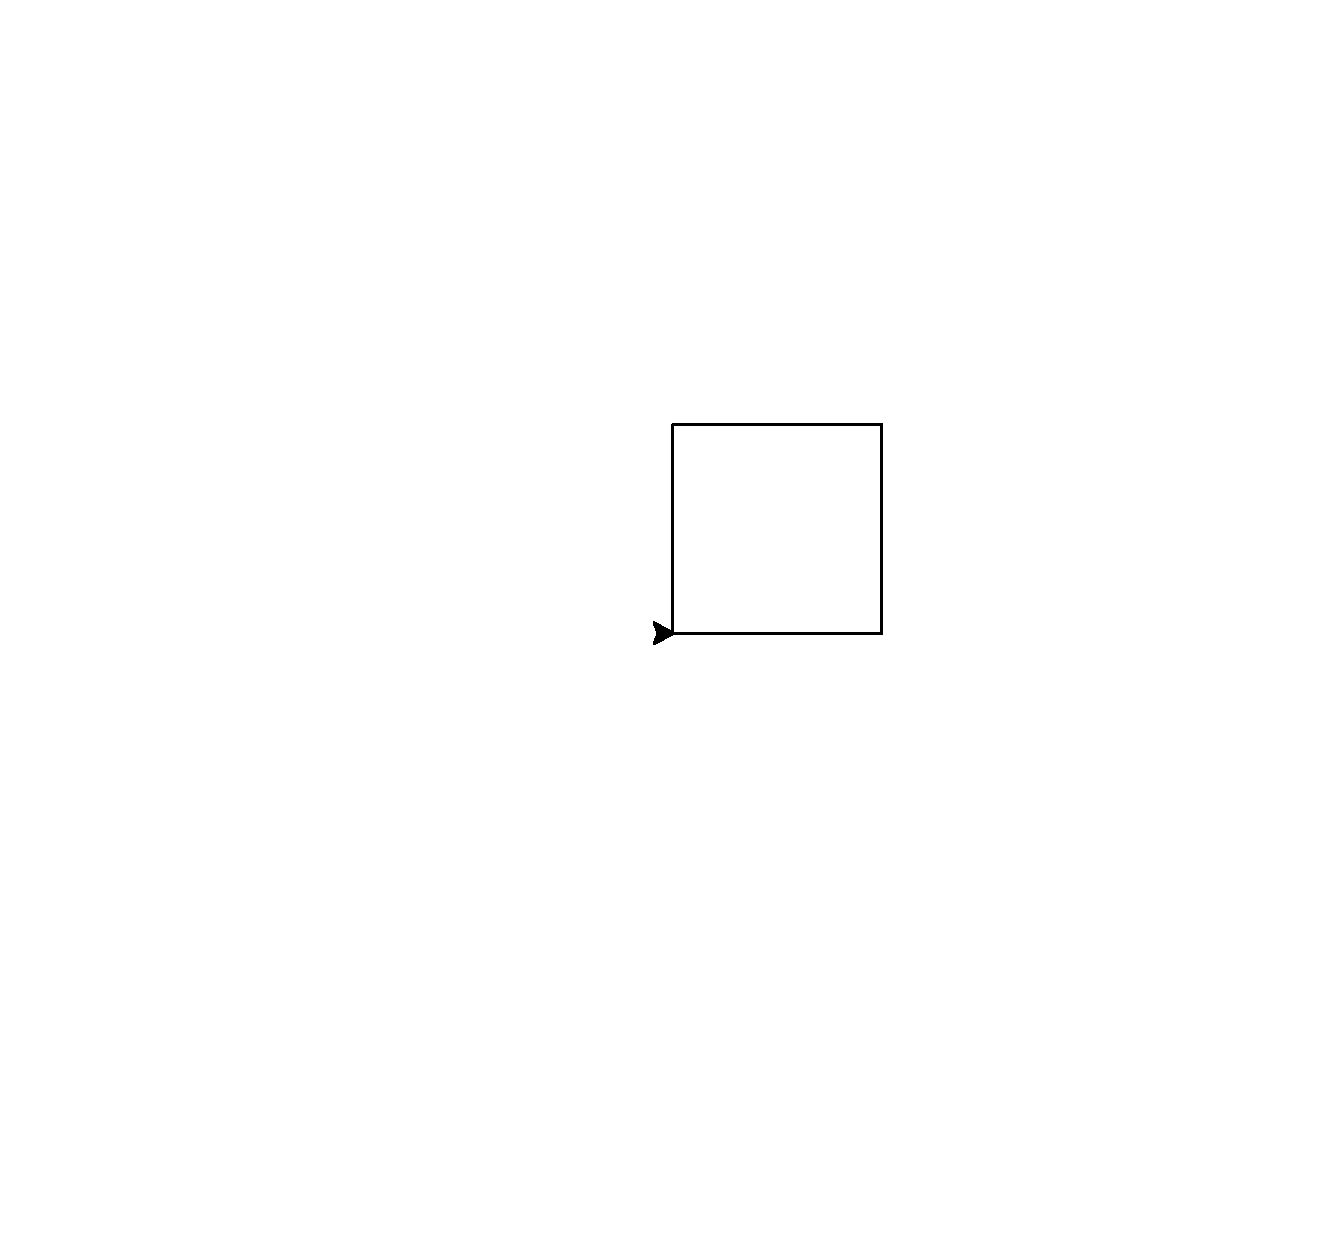
\includegraphics[clip,trim=0 200 0 100, width=\textwidth]{code/Square_Basic.pdf}};
}  

So what are we doing here ?

\begin{itemize}
\item[\pointSymbol]
In line 5, we are adding a property/flag to \code{bob} called \code{busy}. This will store \code{True} when \code{bob} should not be interrupted, and  \code{False} when \code{bob} can be interrupted to  do another task.
 
\item[\pointSymbol]
Then every task that we plan for \code{bob} should have the same structure and \code{drawSquare}. In that we 
\begin{itemize}
\item Check if \code{bob} is \code{busy}, and if yes the return without doing anything.
\item Set property/flag \code{busy} to \code{True} so \code{bob} can't be interrupted.
\item Do the task at hand --- here the task is drawing a square.
\item Once task is finished we need to set property/flag \code{busy} to \code{False} so \code{bob} can be interrupted again.
\end{itemize}
\end{itemize}

\begin{itemize}
\item[\todoSymbol] \color{todo}
Modify the above code so that it prints out a message "I'm busy" whenever \code{bob} is interrupted during drawing a square.
\end{itemize}

\section{TakeAway game ---- remember me ?}\label{sec:game}

OK, we are 8 pages in and we have not started on our TakeAway game yet.  I'm too lazy to change the chapter title so we will leave the game until next week.

\end{document}

\clearpage

\section{TakeAway game ---- remember me ?}\label{sec:game}

OK, we are 8 pages in and we have not started on our TakeAway game yet.  I'm too lazy to change the chapter title so let's see if we can get the game done in one page \ldots


\begin{itemize}
\item[\todoSymbol] \color{todo}

Write an event-based program that
\begin{itemize}
\item
Plays the Take Away game but this time all input/output is via the turtle graphics.

\item Will respond to events
\begin{itemize}
\item On key ``\code{s}'' press the game restarts.  
\item On key ``\code{1}'' press the user takes one coin.
\item On key ``\code{2}'' press the user takes two coins.
\item On key ``\code{3}'' press the user takes three coins.
\item On key ``\code{Q}'' press quit the game. Use \code{bob.bye()} for this.
\end{itemize}

\item 
We will leave the drawing of the coins to another day, instead we will just display the number of coins left using \code{bob.write}.

\end{itemize}

\end{itemize}


\end{document}


